\documentclass{article}

% Preamble from the automatic .tex template in your Neovim init.lua.
\usepackage[english]{babel}
\usepackage[letterpaper,top=2cm,bottom=2cm,left=3cm,right=3cm,marginparwidth=1.75cm]{geometry}
\usepackage{amsmath}
\usepackage{amssymb}
\usepackage{amsthm}
\usepackage{graphicx}
\usepackage{tikz}
\usepackage[colorlinks=true, allcolors=blue]{hyperref}

\definecolor{hyperedgeone}{HTML}{3B6BB2}
\definecolor{hyperedgetwo}{HTML}{C47A18}
\definecolor{hyperedgethree}{HTML}{228B72}

\theoremstyle{definition}
\newtheorem{definition}{Definition}
\theoremstyle{plain}
\newtheorem{proposition}{Proposition}

\title{Hypershift: Lead Lag Inference}
\author{Hypershift Team} % Add authors here.
\date{\today}

\begin{document}
\maketitle

\begin{abstract}
% Write your abstract here.
\end{abstract}

% Uncomment if you want a table of contents while drafting.
% \tableofcontents

\section{Introduction}
% Write your paper here. Add sections as needed with \section{Title}.

% References can stay in this file, as in your Neovim template.
% Uncomment and add real entries when you are ready to cite sources.
% \begin{thebibliography}{9}
% \bibitem{key}
% Author. \textit{Title}. Source, year.
% \end{thebibliography}

\section{Related Work and Relationship to THINK}

\section{Forecasting Problem and Data}

\section{Mathematical Foundations}

\subsection{Hypergraphs and Incidence Representations}
\begin{definition}[Hypergraph]
\label{def:hypergraph}
A \emph{finite hypergraph} is a pair
\[
  \mathcal{H} = (V,E),
  \qquad E \subseteq 2^V \setminus \{\varnothing\},
\]
where $V$ is a finite, nonempty set of \emph{vertices} and $E$ is a
collection of nonempty subsets of $V$, called \emph{hyperedges}.
Here, $2^V$ denotes the power set of $V$. A hyperedge may contain any
number of vertices; an ordinary simple graph is the special case in which
every hyperedge contains exactly two vertices.
\end{definition}

\begin{definition}[Incidence matrix]
\label{def:incidence-matrix}
Let $\mathcal{H}=(V,E)$ be a finite hypergraph, and fix orderings
$V=\{v_1,\ldots,v_n\}$ and $E=\{e_1,\ldots,e_m\}$, where
$n=|V|$ and $m=|E|$. The \emph{incidence matrix} of $\mathcal{H}$ is
the binary matrix $\mathbf{H}\in\{0,1\}^{n\times m}$ defined by
\[
  H_{ij} =
  \begin{cases}
    1, & \text{if } v_i\in e_j,\\
    0, & \text{otherwise},
  \end{cases}
  \qquad 1\leq i\leq n,\quad 1\leq j\leq m.
\]
Thus, rows correspond to vertices and columns correspond to hyperedges;
the $j$th column records the vertices belonging to $e_j$.
\end{definition}

\paragraph{Example.}
Let $V=\{v_1,v_2,v_3,v_4,v_5\}$ and $E=\{e_1,e_2,e_3\}$, with
\[
  e_1=\{v_1,v_2,v_3\},\qquad
  e_2=\{v_3,v_4,v_5\},\qquad
  e_3=\{v_2,v_4\}.
\]
The hypergraph and its incidence matrix are shown side by side in
Figure~\ref{fig:hypergraph-incidence-example}.

% A nonfloating block keeps the diagram, matrix, and caption in source order.
\par\medskip
\noindent\begin{minipage}{\textwidth}
  \makeatletter
  \def\@captype{figure}
  \makeatother
  \centering
  \begin{minipage}[t]{0.48\textwidth}
    \centering
    \textbf{(a) Hypergraph}\par\medskip
    \parbox[c][4.3cm][c]{\linewidth}{%
      \centering
      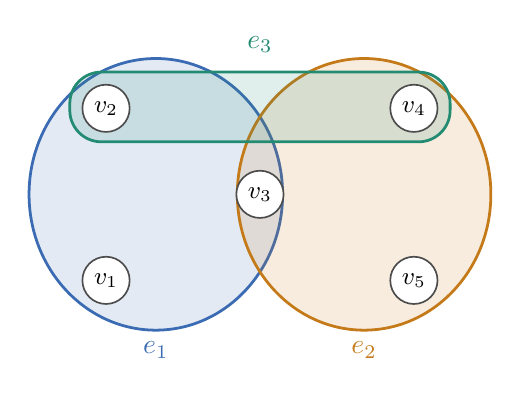
\begin{tikzpicture}[x=1.15cm,y=1.15cm,
        vertex/.style={circle,draw=black!70,fill=white,
          line width=0.6pt,minimum size=6mm,inner sep=1pt,font=\small}]
        % Each shaded region contains exactly the vertices in its hyperedge.
        \draw[draw=hyperedgeone,fill=hyperedgeone,fill opacity=0.14,
          line width=1pt]
          (-1.15,0) ellipse [x radius=1.4,y radius=1.5];
        \draw[draw=hyperedgetwo,fill=hyperedgetwo,fill opacity=0.14,
          line width=1pt]
          (1.15,0) ellipse [x radius=1.4,y radius=1.5];
        \draw[draw=hyperedgethree,fill=hyperedgethree,fill opacity=0.14,
          line width=1pt,rounded corners=4mm]
          (-2.1,0.58) rectangle (2.1,1.35);
        \node[vertex] at (-1.7,-0.95) {$v_1$};
        \node[vertex] at (-1.7,0.95) {$v_2$};
        \node[vertex] at (0,0) {$v_3$};
        \node[vertex] at (1.7,0.95) {$v_4$};
        \node[vertex] at (1.7,-0.95) {$v_5$};
        \node[text=hyperedgeone] at (-1.15,-1.72) {$e_1$};
        \node[text=hyperedgetwo] at (1.15,-1.72) {$e_2$};
        \node[text=hyperedgethree] at (0,1.65) {$e_3$};
      \end{tikzpicture}%
    }
  \end{minipage}\hfill
  \begin{minipage}[t]{0.48\textwidth}
    \centering
    \textbf{(b) Incidence matrix}\par\medskip
    \parbox[c][4.3cm][c]{\linewidth}{%
      \centering
      $\displaystyle
      \mathbf{H}=\bordermatrix{
           & \textcolor{hyperedgeone}{e_1}
           & \textcolor{hyperedgetwo}{e_2}
           & \textcolor{hyperedgethree}{e_3}\cr
        v_1 & 1 & 0 & 0\cr
        v_2 & 1 & 0 & 1\cr
        v_3 & 1 & 1 & 0\cr
        v_4 & 0 & 1 & 1\cr
        v_5 & 0 & 1 & 0\cr
      }$%
    }
  \end{minipage}
  \caption{A hypergraph with five vertices and three hyperedges, together
    with its incidence matrix. Matching colors identify the shaded
    hyperedges and their matrix columns. For example, $v_3$ belongs to both
    $e_1$ and $e_2$, so its row is $(1,1,0)$.}
  \label{fig:hypergraph-incidence-example}
\end{minipage}
\par\medskip

\subsection{Generic Hypergraph Message Passing}
\begin{definition}[Feedforward neural network]

\label{def:feedforward-neural-network}
Let $L \geq 1$ and let $d_0,\ldots,d_L$ be positive integers.
For each $\ell=1,\ldots,L$, let
\[
  W^{(\ell)} \in \mathbb{R}^{d_\ell \times d_{\ell-1}},
  \qquad
  b^{(\ell)} \in \mathbb{R}^{d_\ell}.
\]
For each $\ell=1,\ldots,L-1$, let
\[
  \sigma_\ell :
  \mathbb{R}^{d_\ell} \longrightarrow \mathbb{R}^{d_\ell}
\]
be a fixed activation function applied coordinatewise.

A \emph{fully connected feedforward neural network with an
affine output layer} is a parameterized map
\[
  f_\theta :
  \mathbb{R}^{d_0} \longrightarrow \mathbb{R}^{d_L}
\]
defined, for an input $x \in \mathbb{R}^{d_0}$, by
\[
  h^{(0)} = x,
\]
\[
  h^{(\ell)}
  =
  \sigma_\ell\!\left(
    W^{(\ell)}h^{(\ell-1)} + b^{(\ell)}
  \right),
  \qquad \ell=1,\ldots,L-1,
\]
and
\[
  f_\theta(x)
  =
  W^{(L)}h^{(L-1)} + b^{(L)}.
\]
Here,
\[
  \theta
  =
  \bigl((W^{(\ell)},b^{(\ell)})\bigr)_{\ell=1}^{L}
\]
denotes the collection of trainable parameters.
The vectors $h^{(1)},\ldots,h^{(L-1)}$ are called
\emph{hidden representations}, and
$d_1,\ldots,d_{L-1}$ are the corresponding
\emph{hidden-layer widths}.

\end{definition}

\begin{definition}[Hypergraph neural network (HGNN)]
\label{def:hgnn}
Let $\mathcal{H}=(V,E)$ be a finite hypergraph with vertex features
$x_i\in\mathbb{R}^{d_0}$, and let $E_i=\{e\in E:v_i\in e\}$.
Fix an integer $L\geq1$ for the number of propagation layers.
A \emph{message-passing hypergraph neural network} computes vertex
representations through successive vertex-to-hyperedge and
hyperedge-to-vertex updates.\footnote{For the general two-stage
formulation, see Jing Huang and Jie Yang,
\href{https://www.ijcai.org/proceedings/2021/0353.pdf}{\emph{UniGNN:
a Unified Framework for Graph and Hypergraph Neural Networks}},
IJCAI, 2021.}
Starting from $h_i^{(0)}=x_i$, layer $\ell=1,\ldots,L$ has the form
\begin{align*}
  z_e^{(\ell)}
    &= \Phi^{(\ell)}\!\left(
       \operatorname{AGG}_{V}^{(\ell)}\!\left(
       \{\!\{h_j^{(\ell-1)}:v_j\in e\}\!\}\right)\right),\\
  m_i^{(\ell)}
    &= \operatorname{AGG}_{E}^{(\ell)}\!\left(
       \{\!\{z_e^{(\ell)}:e\in E_i\}\!\}\right),\\
  h_i^{(\ell)}
    &= \Psi^{(\ell)}\!\left(h_i^{(\ell-1)},m_i^{(\ell)}\right).
\end{align*}
Here, $h_i^{(\ell)}\in\mathbb{R}^{d_\ell}$ and
$z_e^{(\ell)},m_i^{(\ell)}\in\mathbb{R}^{s_\ell}$ for positive dimensions
$d_\ell$ and $s_\ell$. The notation $\{\!\{\cdot\}\!\}$ denotes a multiset,
and the aggregation
operators are invariant to permutations of their inputs, as with sums
or means. The trainable maps $\Phi^{(\ell)}$ and $\Psi^{(\ell)}$ are
shared across hyperedges and vertices, respectively, and may be
feedforward networks as in Definition~\ref{def:feedforward-neural-network}.
For an isolated vertex, the hyperedge aggregate is defined to be zero.
A shared trainable readout $\rho:\mathbb{R}^{d_L}\to\mathbb{R}^{d_{\mathrm{out}}}$
produces the prediction $\widehat y_i=\rho(h_i^{(L)})$ for vertex $v_i$.
\end{definition}

The hyperedge transformation used in our Euclidean model is a
feedforward neural network with one hidden layer:
\[
  \Phi_\theta(z)
  =
  W^{(2)}
  \operatorname{ReLU}\!\left(
    W^{(1)}z+b^{(1)}
  \right)
  +b^{(2)},
\]
where $\operatorname{ReLU}(a)=\max\{0,a\}$ is applied
coordinatewise. This network transforms an aggregated
hyperedge representation into a message that is subsequently
distributed to the incident vertices.

\paragraph{Message passing in the current Euclidean model.}
The current implementation performs one vertex-to-hyperedge-to-vertex
round across multiple hyperedge families on the same vertex set.
The equations below describe one input sample; batching applies the
same computation independently to each sample. Let
$x_i\in\mathbb{R}^{d_{\mathrm{in}}}$ be the input representation of
vertex $v_i$, let $a_i\in\{0,1\}$ indicate whether that vertex is
active, and let $d$ be the hidden dimension. First, the shared affine
projection produces
\[
  r_i=P(a_i x_i)+b_P,\qquad
  P\in\mathbb{R}^{d\times d_{\mathrm{in}}},\quad
  b_P\in\mathbb{R}^{d}.
\]
For each enabled family $f\in\mathcal{F}$, let
$\mathbf{H}^{(f)}\in\{0,1\}^{n\times m_f}$ be its supplied incidence
matrix after constructor validity checks, and let $w_j^{(f)}\geq0$
be its hyperedge weights, which default to one. A hyperedge is usable
only when it contains at least two active vertices:
\[
  \delta_j^{(f)}=\sum_{i=1}^{n}a_i H_{ij}^{(f)},\qquad
  u_j^{(f)}=\mathbf{1}\!\left\{\delta_j^{(f)}\geq2\right\}.
\]
Invalid hyperedges supplied by a constructor have zero incidence
columns. For learned families, the membership module supplies binary
forward values and uses a straight-through estimator during training.

The vertex-to-hyperedge step takes an active-vertex mean and applies
the shared feedforward map $\Phi_\theta$ defined above:
\[
  \bar r_j^{(f)}=
    \frac{\sum_{i=1}^{n}a_i H_{ij}^{(f)}r_i}
         {\max\{\delta_j^{(f)},1\}},\qquad
  z_j^{(f)}=u_j^{(f)}\Phi_\theta\!\left(\bar r_j^{(f)}\right).
\]
Both affine layers of this edge transformation map
$\mathbb{R}^{d}$ to $\mathbb{R}^{d}$, and the same transformation is
used for every hyperedge in every family. The hyperedge-to-vertex step
then returns a weighted message. With the default family normalization,
\begin{align*}
  d_i^{(f)}
    &= a_i\sum_{j=1}^{m_f}H_{ij}^{(f)}u_j^{(f)}w_j^{(f)},\\
  m_i^{(f)}
    &= \frac{a_i}{\max\{d_i^{(f)},1\}}
       \sum_{j=1}^{m_f}H_{ij}^{(f)}w_j^{(f)}z_j^{(f)}.
\end{align*}
The denominator implements the code's degree clamp at one. Disabling
family normalization replaces this denominator by one, giving an
unnormalized weighted sum. Inactive vertices receive zero family
messages.

Each family has a learned scalar logit $\lambda_f$. For vertex $v_i$,
define the available families by
$\mathcal{F}_i=\{f\in\mathcal{F}:d_i^{(f)}>0\}$. Their mixing weights are
\[
  \alpha_i^{(f)}=
  \begin{cases}
    \displaystyle\frac{\exp(\lambda_f)}
      {\sum_{g\in\mathcal{F}_i}\exp(\lambda_g)},
      & f\in\mathcal{F}_i,\\[6pt]
    0, & \text{otherwise}.
  \end{cases}
\]
All logits start at zero, so the initial mixture is uniform over the
available families. These logits are shared across vertices; their
normalization depends on each vertex's family availability.

Finally, the mixed messages are added to the direct representation,
and a shared affine head produces the prediction:
\[
  h_i=r_i+\sum_{f\in\mathcal{F}}\alpha_i^{(f)}m_i^{(f)}
      +C(q\odot\eta),\qquad
  \widehat y_i=W_{\mathrm{out}}h_i+b_{\mathrm{out}}.
\]
Here, $q$ is an optional sample-level context vector, $\eta$ is its
coordinatewise validity mask, $\odot$ denotes elementwise multiplication,
and $C$ is a learned linear projection without a bias. The context term
is omitted when context is disabled. If no family is available to a
vertex, every mixing weight is zero and the direct pathway is retained.
The output dimension defaults to one. These updates correspond to
\texttt{HyperedgeConsumer} in \texttt{src/hypergraph.py}, with runtime
incidence masking supplied by \texttt{hyperedges/common/runtime.py}.

\subsection{Metric Spaces and Gromov Hyperbolicity}

\begin{definition}[Metric space]
\label{def:metric-space}
A \emph{metric space} is a pair $(X,d)$, where $X$ is a nonempty set
and $d:X\times X\to[0,\infty)$ satisfies, for all $x,y,z\in X$,
\[
  \begin{aligned}
    &d(x,y)\geq0
      &&\text{(nonnegativity)},\\
    &d(x,y)=0\ \Longleftrightarrow\ x=y
      &&\text{(identity of indiscernibles)},\\
    &d(x,y)=d(y,x)
      &&\text{(symmetry)},\\
    &d(x,z)\leq d(x,y)+d(y,z)
      &&\text{(triangle inequality)}.
  \end{aligned}
\]
The value $d(x,y)$ is the distance between $x$ and $y$; it is always
finite under this definition.
\end{definition}

\begin{definition}[Vertex $s$-walk distance]
\label{def:s-walk-metric}
Let $\mathcal{H}=(V,E)$ have binary incidence matrix $\mathbf{H}$,
and fix an integer $s\geq1$. The number of hyperedges shared by two
vertices is
\[
  c_{ij}=(\mathbf{H}\mathbf{H}^{\top})_{ij}
        =\sum_{k=1}^{m}H_{ik}H_{jk}
        =\bigl|\{e\in E:v_i,v_j\in e\}\bigr|.
\]
Define the undirected, unweighted graph $G_s=(V,F_s)$ by its adjacency
matrix
\[
  (A_s)_{ij}=
  \begin{cases}
    1, & i\neq j\ \text{and }c_{ij}\geq s,\\
    0, & \text{otherwise}.
  \end{cases}
\]
A \emph{vertex $s$-walk} is a sequence $W=(u_0,\ldots,u_\ell)$
whose consecutive vertices are adjacent in $G_s$. Its length is
$\operatorname{len}(W)=\ell$, so each graph step has unit length.
On a nonempty connected component $C\subseteq V$ of $G_s$, define
\begin{equation}
  \label{eq:s-walk-distance}
  d_s(x,y)=\min\{\operatorname{len}(W):
                W\text{ is an }s\text{-walk from }x\text{ to }y\},
  \qquad x,y\in C.
\end{equation}
The length-zero walk from a vertex to itself is allowed. Thus $d_s$
is precisely the shortest-path distance on the component $C$.
\end{definition}

The routine \texttt{s\_walk\_adjacency} in
\texttt{hyperbolicity/core.py} implements this convention.
The primary structural diagnostic concatenates the family incidence
matrices, removes duplicate columns, and retains hyperedges of size at
least two before forming $A_s$. Its shared-edge counts therefore refer
to distinct retained hyperedges. If $G_s$ is disconnected, there is no
finite walk between different components. The componentwise diagnostic
in \texttt{hyperbolicity/diagnostics.py} evaluates each component
separately; the core shortest-path routine rejects a disconnected input.

\begin{proposition}[$s$-walk distance is a metric]
\label{prop:s-walk-metric}
For every nonempty connected component $C$ of $G_s$, the pair
$(C,d_s)$ is a metric space.
\end{proposition}

\begin{proof}
Connectedness guarantees a finite walk between any $x,y\in C$.
The possible walk lengths form a nonempty subset of the nonnegative
integers, so a shortest walk exists and $d_s(x,y)$ is finite.
Every length is nonnegative, establishing nonnegativity.

The length-zero walk gives $d_s(x,x)=0$. Conversely, a length-zero
walk has only one vertex, so $d_s(x,y)=0$ implies $x=y$.
This establishes identity of indiscernibles.

Since $\mathbf{H}\mathbf{H}^{\top}$ is symmetric, adjacency in $G_s$
is symmetric. Reversing any walk preserves its length. Reversing a
shortest walk in each direction therefore gives $d_s(x,y)=d_s(y,x)$.

Finally, concatenate a shortest walk from $x$ to $y$ with one from
$y$ to $z$. This is an $s$-walk from $x$ to $z$ of length
$d_s(x,y)+d_s(y,z)$. Minimality of the shortest walk from $x$ to $z$
implies
\[
  d_s(x,z)\leq d_s(x,y)+d_s(y,z),
\]
which is the triangle inequality. All four metric axioms hold.
\end{proof}

\begin{definition}[Gromov product and Gromov hyperbolicity]
\label{def:gromov-hyperbolicity}
Let $(X,d)$ be a metric space. For $x,y,o\in X$, the
\emph{Gromov product} of $x$ and $y$ based at $o$ is
\[
  (x\mid y)_o=\frac{d(x,o)+d(y,o)-d(x,y)}{2}.
\]
For $\delta\geq0$, the space is \emph{$\delta$-hyperbolic} if
\begin{equation}
  \label{eq:gromov-product-inequality}
  (x\mid z)_o\geq
  \min\{(x\mid y)_o,(y\mid z)_o\}-\delta
  \qquad\text{for all }x,y,z,o\in X.
\end{equation}
Its \emph{Gromov hyperbolicity constant} is
\[
  \delta(X,d)=\inf\{\delta\geq0:
                  \text{inequality~\eqref{eq:gromov-product-inequality}
                  holds for all }x,y,z,o\in X\}.
\]
The space is \emph{Gromov hyperbolic} when this constant is finite.
The convention here quantifies over every base point $o$ and gives
the four-point constant used by the implementation.\footnote{See
Herv\'e Fournier, Anas Ismail, and Antoine Vigneron,
\href{https://webusers.imj-prg.fr/~herve.fournier/publications/hyperbolicity.pdf}{\emph{Computing
the Gromov hyperbolicity of a discrete metric space}}, Section~1.1.}
\end{definition}

\begin{definition}[Relative hyperbolicity score]
\label{def:relative-hyperbolicity}
For a finite metric space $(X,d)$, let
\[
  D=\operatorname{diam}(X,d)=\max_{x,y\in X}d(x,y).
\]
When $D>0$, the diameter-normalized score used in this project is
\begin{equation}
  \label{eq:relative-hyperbolicity}
  \boxed{\operatorname{rel}(X,d)
    =\delta_{\mathrm{rel}}(X,d)
    =\frac{2\delta(X,d)}{\operatorname{diam}(X,d)}.}
\end{equation}
If $D=0$, this score is undefined, matching the \texttt{None} returned
by \texttt{relative\_delta}.
\end{definition}

For the structural metric, these definitions apply to $(C,d_s)$.
Feature-space hyperbolicity uses its own feature distance matrix and
diameter; in the dataset summary, \texttt{delta\_hg} is structural,
whereas \texttt{delta\_rel} normalizes the feature-space constant.
The componentwise structural diagnostic also reports a normalized
structural constant using the same formula.

\paragraph{Derivation of the four-point analytic formula.}
For four points $x,y,z,w\in X$, define the three opposite-pair sums
\begin{align*}
  S_1&=d(x,y)+d(z,w),\\
  S_2&=d(x,z)+d(y,w),\\
  S_3&=d(x,w)+d(y,z).
\end{align*}
Write $S_{(1)}\leq S_{(2)}\leq S_{(3)}$ for these values in sorted
order, including ties.

\begin{proposition}[Four-point formula]
\label{prop:four-point-formula}
The smallest constant satisfying
\eqref{eq:gromov-product-inequality} for all orderings of this quadruple is
\begin{equation}
  \label{eq:four-point-delta}
  \boxed{\delta_4(x,y,z,w)=\frac{S_{(3)}-S_{(2)}}{2}
    =\frac{\max\{S_1,S_2,S_3\}-\operatorname{med}\{S_1,S_2,S_3\}}{2}.}
\end{equation}
Consequently, for a finite metric space,
\begin{equation}
  \label{eq:global-four-point-delta}
  \boxed{\delta(X,d)=\max_{x,y,z,w\in X}\delta_4(x,y,z,w).}
\end{equation}
\end{proposition}

\begin{proof}
Use $w$ as the base point and set
$T=d(x,w)+d(y,w)+d(z,w)$. Substituting the definitions gives
\[
  2(x\mid y)_w=T-S_1,\qquad
  2(x\mid z)_w=T-S_2,\qquad
  2(y\mid z)_w=T-S_3.
\]
Multiplying \eqref{eq:gromov-product-inequality} by two therefore gives
\begin{align*}
  T-S_2
    &\geq\min\{T-S_1,T-S_3\}-2\delta\\
    &=T-\max\{S_1,S_3\}-2\delta,
\end{align*}
or, equivalently,
\[
  S_2\leq\max\{S_1,S_3\}+2\delta.
\]
Permuting $x,y,z$ places each of the three sums on the left-hand side.
The inequalities for the smallest and middle sums hold automatically
when $\delta\geq0$. The remaining inequality is exactly
\[
  S_{(3)}\leq S_{(2)}+2\delta
  \quad\Longleftrightarrow\quad
  \delta\geq\frac{S_{(3)}-S_{(2)}}{2}.
\]
This proves \eqref{eq:four-point-delta}. The condition must hold for
every quadruple in $X$, so taking the maximum proves
\eqref{eq:global-four-point-delta}.
\end{proof}

An equivalent formula without a median operation follows from
$S_{(2)}=S_1+S_2+S_3-S_{(1)}-S_{(3)}$:
\[
  \delta_4=\frac{1}{2}\left(
    2\max\{S_1,S_2,S_3\}+\min\{S_1,S_2,S_3\}
    -(S_1+S_2+S_3)\right).
\]
In particular, when $D>0$,
\[
  \boxed{\operatorname{rel}(X,d)
    =\frac{\max_{x,y,z,w\in X}\bigl(S_{(3)}-S_{(2)}\bigr)}{D}.}
\]
Rescaling every distance by $c>0$ rescales every pairing sum,
$\delta(X,d)$, and $D$ by $c$, so $\operatorname{rel}(X,cd)
=\operatorname{rel}(X,d)$. The triangle inequality implies that each
pairing sum is at most the sum of the other two. Thus
$S_{(3)}\leq S_{(1)}+S_{(2)}\leq2S_{(2)}$ and $S_{(3)}\leq2D$,
giving $S_{(3)}-S_{(2)}\leq D$. Therefore
\[
  0\leq\delta(X,d)\leq\frac{D}{2},\qquad
  0\leq\operatorname{rel}(X,d)\leq1.
\]
A tree metric has equal largest pairing sums for every quadruple and
hence $\delta=0$.

The function \texttt{four\_point\_delta} computes
\eqref{eq:four-point-delta} by sorting the three sums.
Repeated points contribute zero by the triangle inequality, so the
exact routine \texttt{exact\_delta\_details} only needs to enumerate
four distinct points; spaces with fewer than four points have
$\delta=0$. A maximum over sampled quadruples is a lower bound on the
exact constant. Its normalized version still uses the full diameter
of the metric space being evaluated.

\subsection{Smooth Manifolds and Tangent Spaces}

\subsection{Riemannian Metrics, Length, and Distance}

\subsection{Geodesics and Exponential and Logarithmic Maps}

\subsection{Specialization to the Poincar\'e Ball}

\section{Model and Hyperedge Construction}

\section{Hyperbolic Geometry and Attention}

\section{Results}

\section{Discussion and Limitations}

\section{Conclusion}

\end{document}
